Though recent advancements in serverless computing has been instrumental in improving the ability of teams to more rapidly develop software, significant challenges remain in the development of cutting edge applications and products in our current compute landscape.
An demonstrative problem domain with this challenge are those characterized by applications that include sophisticated AI pipelines on their critical path.

\begin{figure}[tb]
    \centering
    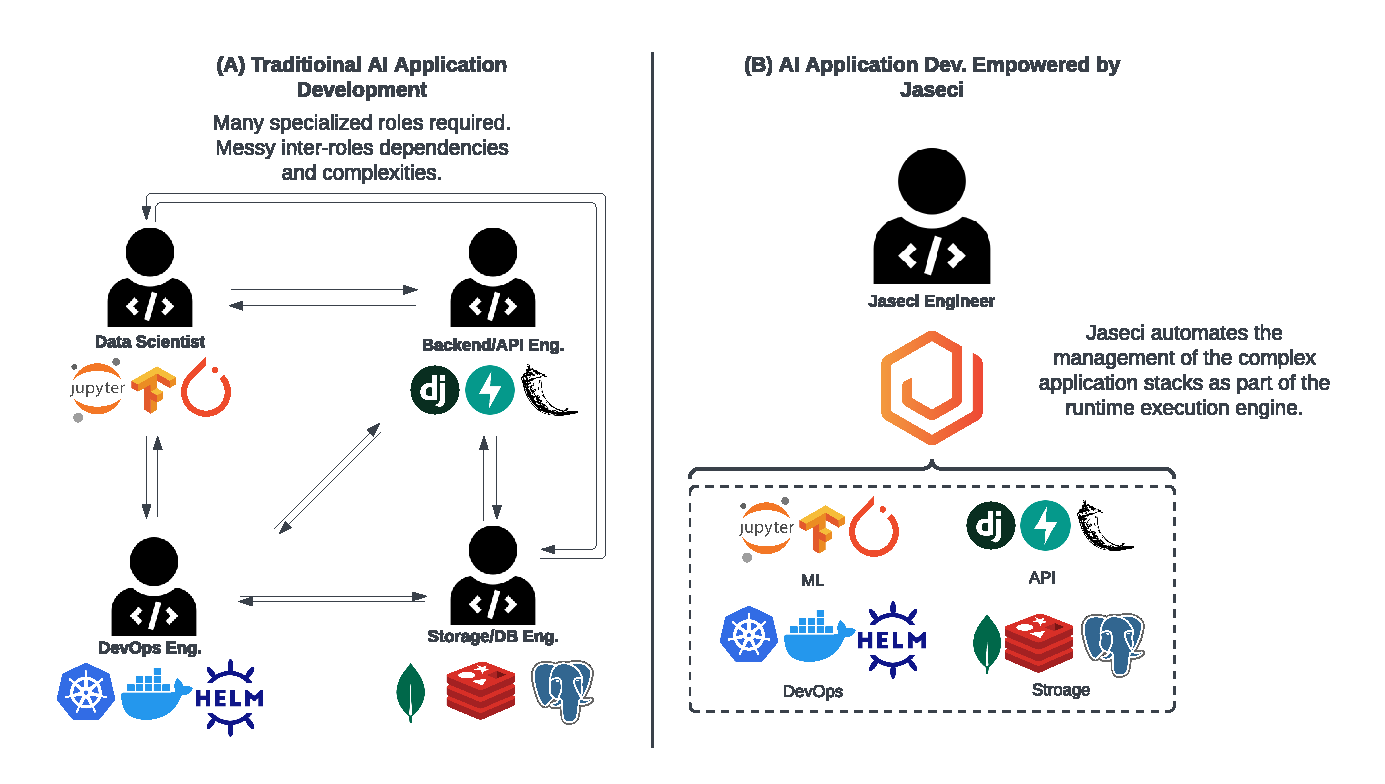
\includegraphics[width=\linewidth]{figures/team_sizes.pdf}
    \caption{Comparison of typical development team required to realize production grade AI application today (left), and the ability of a single software developer to realize such an application with Jaseci (right). }
    \label{fig:dev}
\end{figure}


\subsection{Problem Scenario}
Figure~\ref{fig:dev}A shows the typical set of  often siloed roles needed to create software in this environment.
The first critical role needed is an \emph{architect / tech-lead} responsible for architecting the software solution across disparate components, programming languages, frameworks, and SDKs.
If a microservice ecosystem is needed (which is a must for modern
AI applications), the architect will also decide what will and won't be its own service (container) and define the interfaces between these disparate  services.
For the AI model work, the role of a \emph{data scientist / ML engineer} is needed.
This role typically works primarily in Jupyter notebooks selecting, creating, training and tuning ML models to support application features.
Production software engineering is typically outside of the scope of this expertise in practice.
The role of a \emph{backend engineer} is needed for implementing the main services of the application and taking the code out of Jupyter notebooks to build the models into the backend (server-side) of the application.
The \emph{backend engineer} is also responsible for supporting new features and creating their API interfaces for \emph{frontend} engineers.
One of the key roles any software team needs to deploy an AI product is a \emph{DevOps engineer}.
This role is solely responsible for deploying and configuring containers to run on a cloud and ensure these containers are operational and scaled to the load requirements of the software.
This responsibility covers configuring software instance pods, database pods, caching layers, logging services, and parameterizing replicas and auto-scaling heuristics.



In this traditional model of software engineering, many challenges and complexity emerge.
An example is the (quite typical) scenario of the first main server-side implementation of the application being a monoservice while DB, caching, and logging are microservices.
As the \emph{ML engineer} introduces models of increasing size, the \emph{dev-ops} person alerts the team that the cloud instances, though designated as \emph{large}, only have 8gb of ram.
Meanwhile new AI models being integrated exceed this limit.
This event leads to a re-architecture of the main monoservice to be split out AI models into microservices and interfaces being designed or adopted leading to significant backend work / delays.
In this work, we aim to create a solution that would move all of this decisioning and work under the purview of the automated runtime system.

Ultimately, the mission of Jaseci is to accelerate and democratize the development and deployments of end-to-end scalable AI applications as presented in Figure~\ref{fig:dev}B.
To this end, we present a novel set of higher level abstractions for programming sophisticated software in a micro-service/serverless AI and a full stack architecture and programming model that abstracts away and automates much of the complexity of building diffuse applications on a distributed compute substrate of potentially thousands of compute nodes.